\documentclass[12pt, a4paper]{article}

% Packages dependencies
\usepackage[brazil]{babel}
\usepackage[top=3cm, bottom=2cm, left=3cm, right=3cm]{geometry}
\usepackage{graphicx}
\usepackage{titlesec}
\usepackage{float}
\usepackage{minted}
\usepackage{xcolor}
\usepackage[labelformat=empty]{caption}
\usepackage{amsmath}
\usepackage{amssymb}
\usepackage{multicol}
\usepackage{indentfirst}
\usepackage{hyperref}
\usepackage{titlesec}
\usepackage{enumitem}
\usepackage[most]{tcolorbox}
\usepackage{cleveref}
\usepackage{fontspec}
\hypersetup{
    colorlinks=true,
    urlcolor=blue,
    linkcolor=blue
}
\setmainfont{ARIAL.TTF}[
  ItalicFont = ARIALI.TTF,
  BoldFont = ARIALBD.TTF,
  BoldItalicFont = ARIALBI.TTF,
  Path = ./fontes/
]
\setmonofont{JetBrains Mono}[
Scale=MatchLowercase,
Ligatures=TeX,
Contextuals=Alternate
]
\newtcolorbox{mybox}[2][]{breakable,sharp corners, skin=enhancedmiddle jigsaw,parbox=false,
boxrule=0mm,leftrule=2mm,boxsep=0mm,arc=0mm,outer arc=0mm,attach title to upper,
after title={.\ }, coltitle=black,colback=gray!10,colframe=black, title={#2},
fonttitle=\bfseries,#1}
\renewcommand*\contentsname{SUMÁRIO}

\graphicspath{{images/}}

%Preamble
\date{\today}

%Variable Student Name
\newcommand\studentName{Matheus de Freitas Weber}
\newcommand\studentTwoName{Gabriel Berwanger Silveira}
\newcommand\studentThreeName{Aluno 3}
\newcommand\studentFourName{Aluno 4}

%Variable Course Name
\newcommand\courseName{Circuitos microprocessados}

%Variable Article Name
\newcommand\titleName{Exercício - Aula 04}

%Variable Article SubName
\newcommand\subTitleName{Conversor A/D}

%Variable Teacher Name
\newcommand\teacherName{Jean Schmith}

%Body
\begin{document}

% -- Unisinos title -- %
\begin{center}
	\MakeUppercase{\textbf{Universidade do Vale do Rio dos Sinos (Unisinos)}}

	% -- Course Name -- %
	\MakeUppercase{\textbf{Graduação em Engenharia de controle e automação}} \\[16ex]


	% -- Student Name -- %
	\MakeUppercase{\textbf{\studentName}}
	\\
	\MakeUppercase{\textbf{\studentTwoName}}
	\\[16ex]

	% -- Work Title -- %
	\MakeUppercase{\textbf{\titleName}}

	\textbf{\subTitleName}

	\vfill

	\textbf{São Leopoldo}

	\textbf{2025}

	\thispagestyle{empty}
\end{center}
\newpage

% -- Capa -- %
\begin{center}
	% -- Capa -- %
	\vspace*{28ex}
	\MakeUppercase{\studentName}
	\\
	\MakeUppercase{\studentTwoName}
	\vspace*{16ex}

	\MakeUppercase{\textbf{\titleName}}

	\textbf{\subTitleName}

	\vspace*{8ex}

	% -- Description of the work -- %
	\hfill\begin{minipage}{0.5\linewidth}
		Trabalho apresentado para a matéria {\courseName} pelo Curso de Engenharia de Controle e Automação e Engenharia da Computação da Universidade do Vale do Sinos (UNISINOS), ministrada pelo Prof.\teacherName.
	\end{minipage}
	\vfill

	\textbf{São Leopoldo}

	\textbf{2025}

\end{center}
\thispagestyle{empty}
\setcounter{page}{1}

\newpage
% -- Summary -- %
\begin{center}
	\tableofcontents
\end{center}
\thispagestyle{empty}

\newpage
% -- Introduction -- %
\section{Introdução}
A comunicação serial entre microcontroladores é uma técnica fundamental em sistemas embarcados, permitindo a troca eficiente de dados entre dispositivos. A arquitetura Cliente-Servidor é amplamente utilizada para organizar essa comunicação, onde um dispositivo atua como cliente, solicitando serviços ou dados, enquanto o outro atua como servidor, respondendo às solicitações do cliente. Este trabalho tem como objetivo implementar um sistema de comunicação serial entre dois microcontroladores utilizando a arquitetura Cliente-Servidor, com o intuito de controlar e monitorar o estado de LEDs através de botões físicos.


\newpage
% -- Teorical foundation -- %

\newpage
\section{Metodologia}
\subsection{Materiais Utilizados}
\begin{itemize}
	\item 1x Placas Arduino Uno
	\item 1x Protoboard
	\item 1x Resistores de 220 ohms
	\item 1x Fotoresistor (LDR)
	\item Fios de conexão (jumpers)
	\item Computador com software Arduino IDE instalado
\end{itemize}

\subsection{Diagrama de Conexões}
\begin{figure}[H]
	\centering
	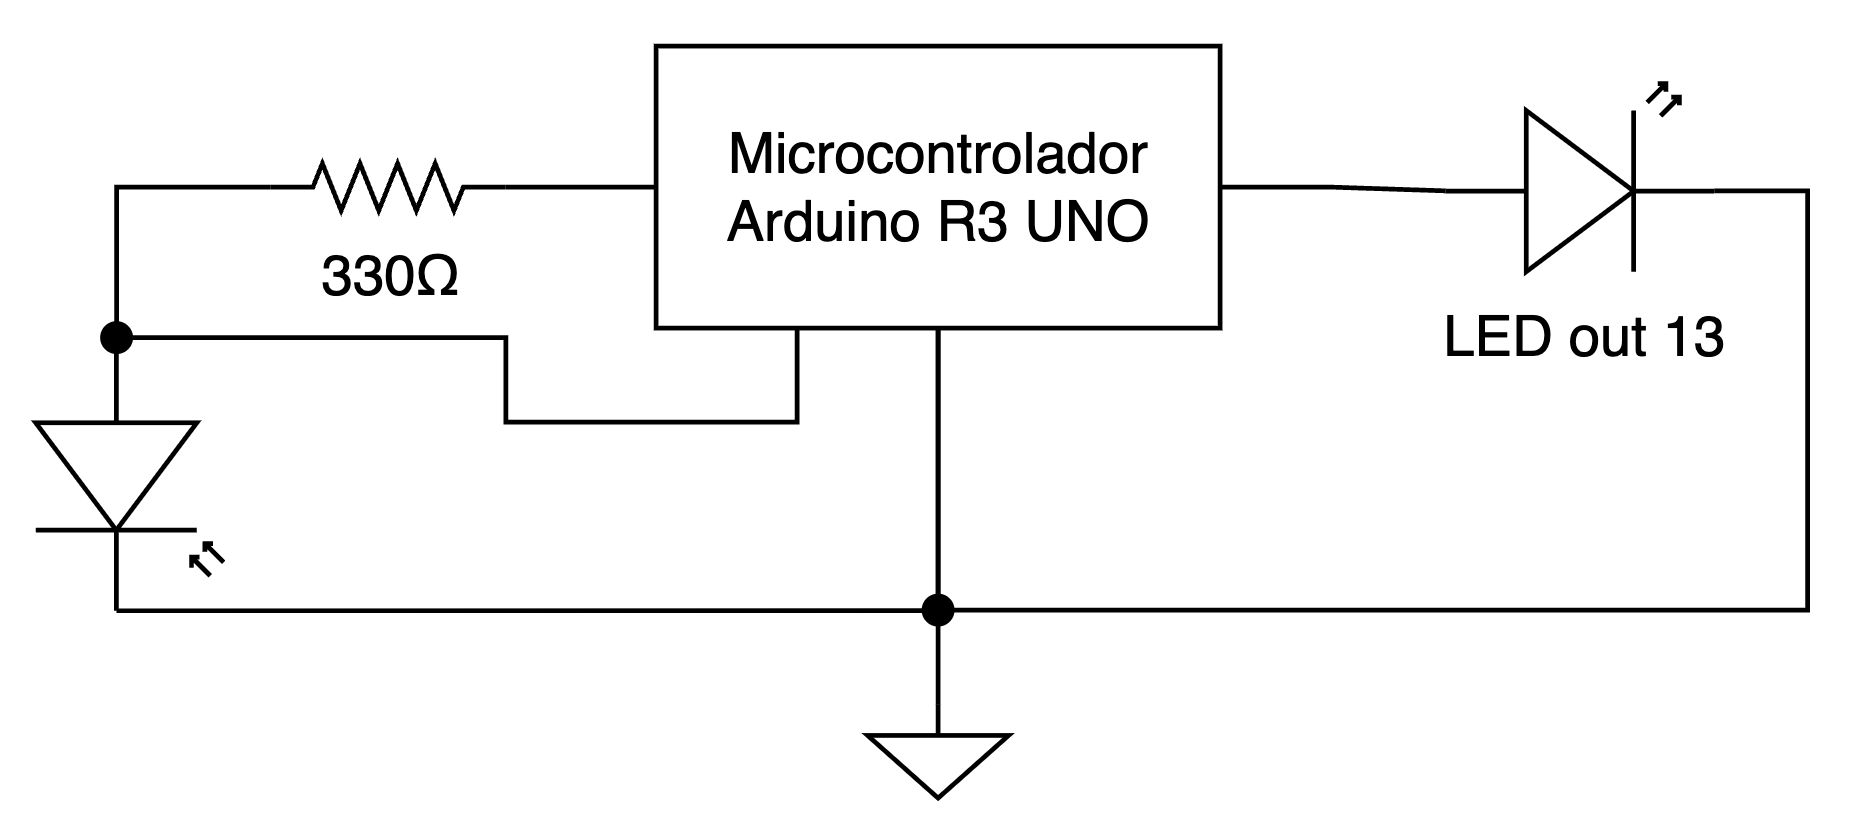
\includegraphics[width=0.8\textwidth]{diagrama_aula04.png}
	\caption{Diagrama de conexões entre os componentes e o Arduino Uno.}
	\label{fig:diagrama_conexoes}
\end{figure}
\begin{figure}[H]
	\centering
	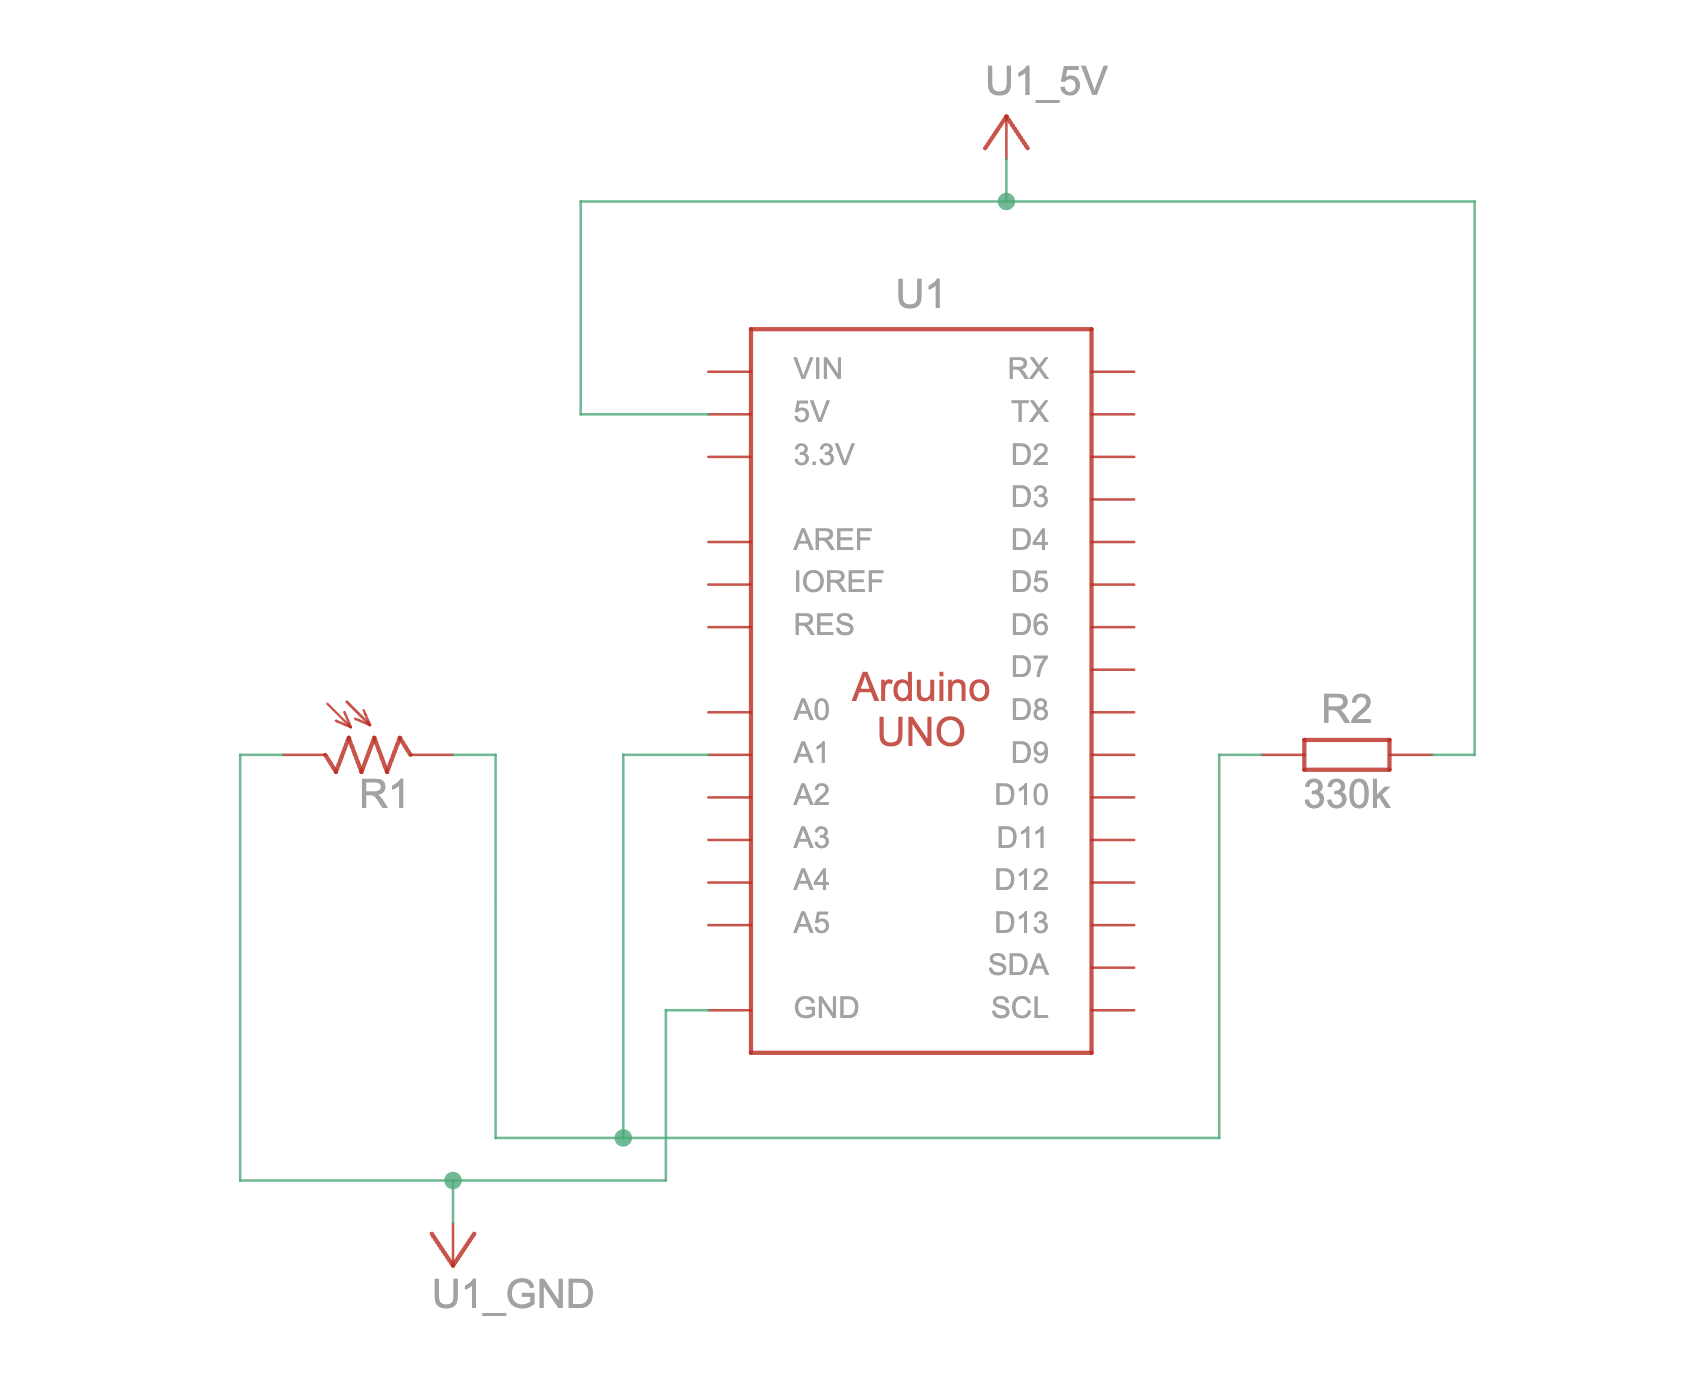
\includegraphics[width=0.8\textwidth]{diagrama_tinkercad_aula03.png}
	\caption{Montagem no TinkerCAD.}
	\label{fig:montagem_protoboard}
\end{figure}

\subsection{Fluxograma}
\begin{figure}[H]
	\centering
	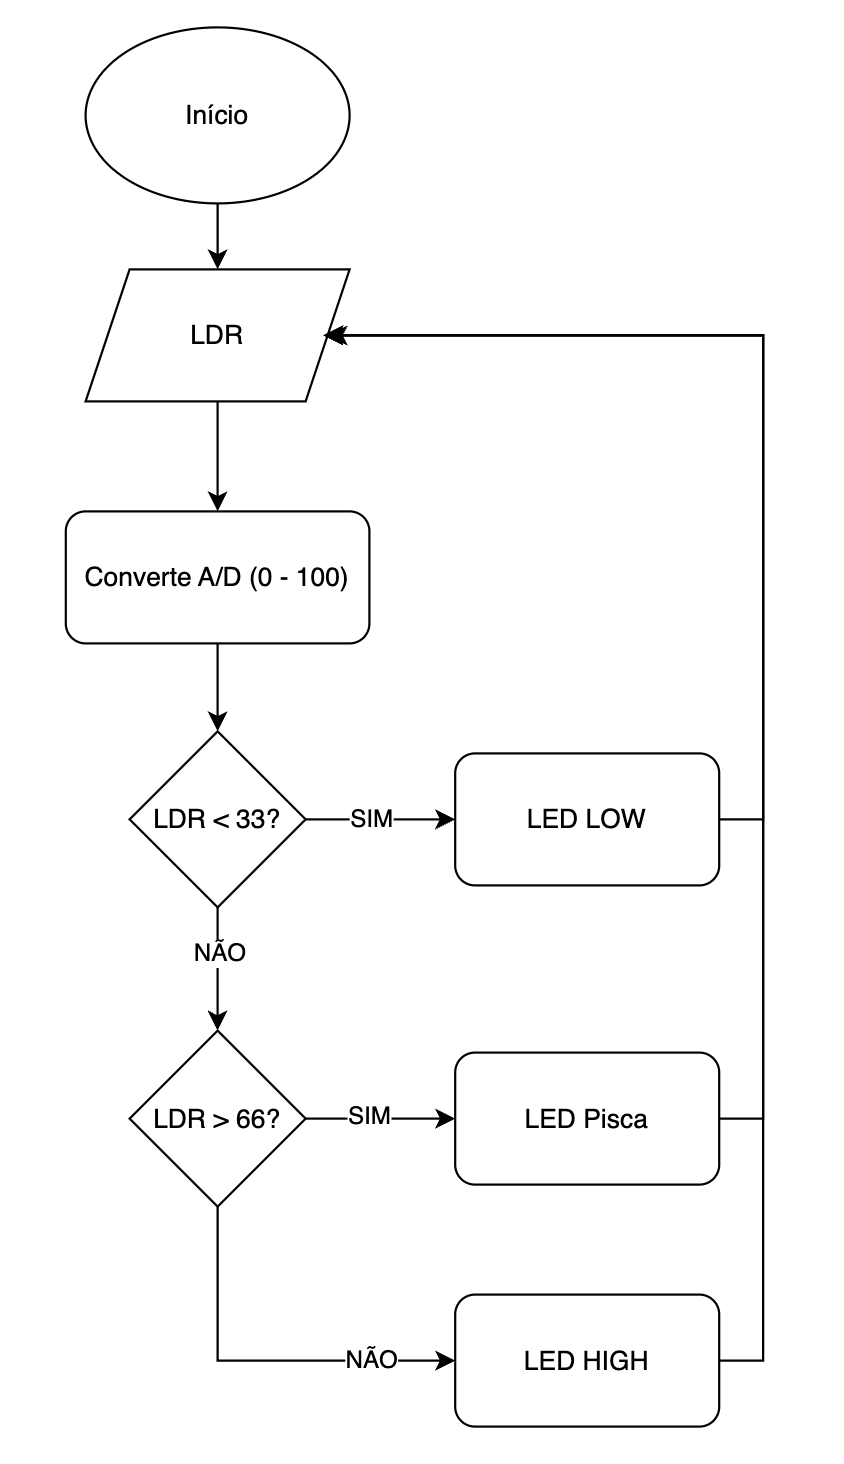
\includegraphics[width=0.8\textwidth]{fluxograma_trabalho_03.png}
	\caption{Fluxograma do funcionamento do sistema.}
	\label{fig:fluxograma_sistema}
\end{figure}

\subsection{Código Fonte}

\begin{mybox}[label={lst:codigo_servidor},title={Código}]{}
	\inputminted[fontsize=\footnotesize,breaklines,linenos]{cpp}{./arduino/main.ino}
\end{mybox}
\section{Resultados}
O conversor A/D foi implementado com sucesso utilizando o microcontrolador Arduino Uno. A leitura analógica do fotoresistor (LDR) foi realizada na porta A1, e os valores foram mapeados para uma escala de 0 a 100. Com base nesses valores, o estado do LED conectado ao pino 13 foi controlado conforme as seguintes condições:
\begin{itemize}
	\item Se o valor lido for menor que 33, o LED será desligado.
	\item Se o valor lido estiver entre 33 e 66, o LED será ligado.
	\item Se o valor lido for maior que 66, o LED piscará.
\end{itemize}
O sistema respondeu adequadamente às variações de luz detectadas pelo LDR, demonstrando a eficácia do conversor A/D na leitura de sinais analógicos e no controle do estado do LED.
\begin{figure}[H]
	\centering
	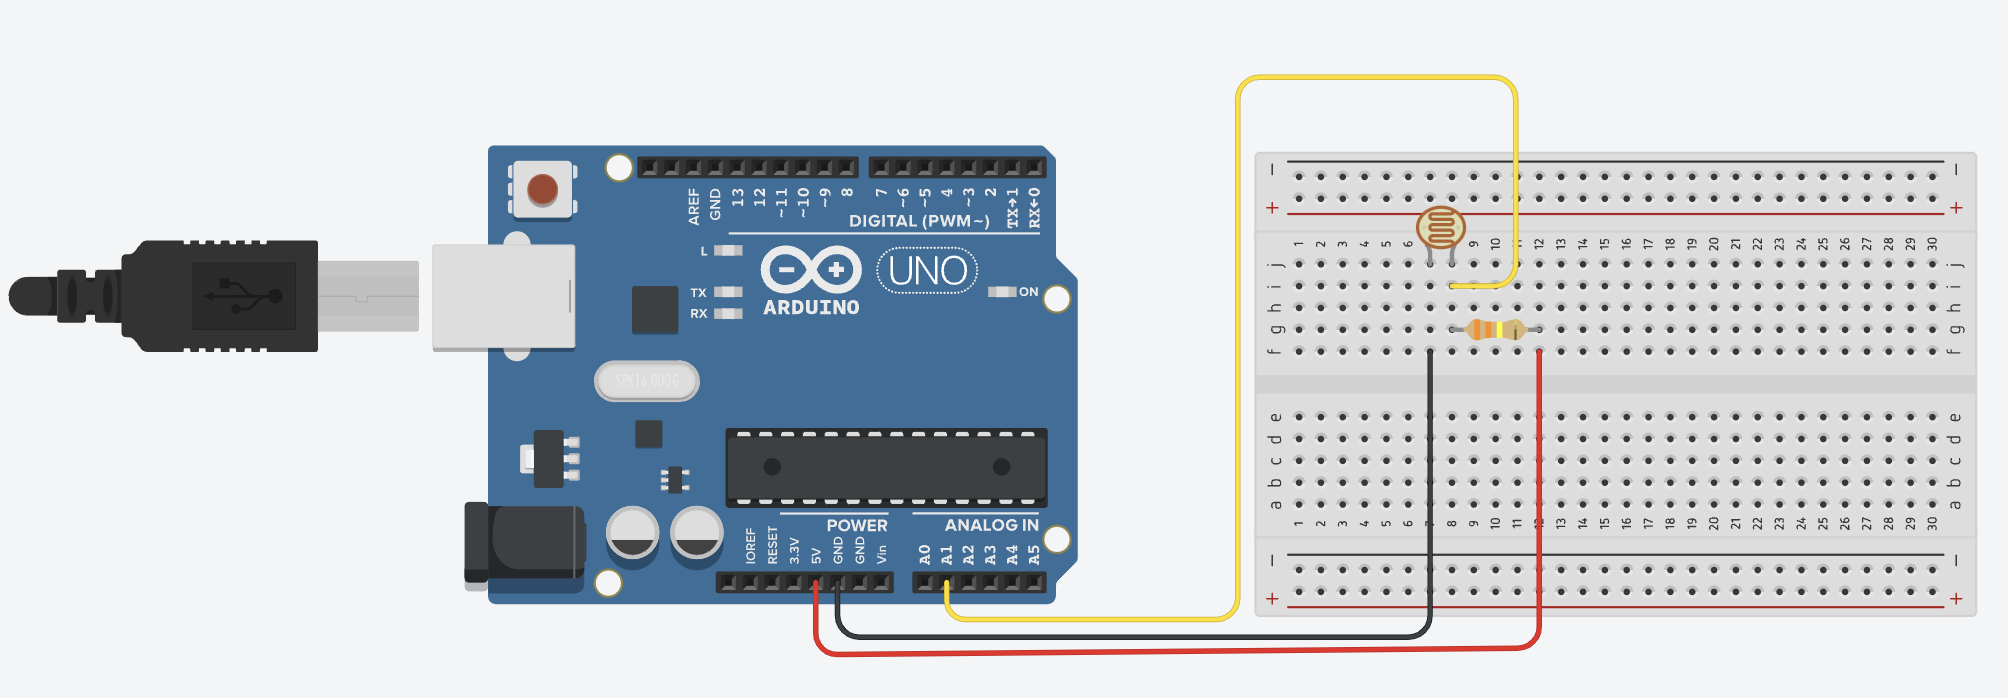
\includegraphics[width=0.8\textwidth]{montagem_aula04.png}
	\caption{Resultado da leitura analógica e controle do LED.}
	\label{fig:resultado_leitura}
\end{figure}

\newpage
% -- Conclusion -- %
\begin{center}
	\section{Conclusão}
\end{center}
O projeto de conversor A/D utilizando o microcontrolador Arduino Uno foi concluído com sucesso, demonstrando a capacidade do sistema em ler sinais analógicos e controlar dispositivos digitais com base nessas leituras. A implementação mostrou-se eficaz para aplicações que requerem monitoramento de variáveis ambientais, como luminosidade, e controle de atuadores, como LEDs. Futuramente, este sistema pode ser expandido para incluir múltiplos sensores e atuadores, além de integrar comunicação com outros dispositivos para aplicações mais complexas em sistemas embarcados.

\rule{\textwidth}{0.4pt}
\subsubsection{Link do TinkerCAD}
\url{https://www.tinkercad.com/things/3dWNFKCmIui-epic-habbi-bigery/editel?returnTo=https%3A%2F%2Fwww.tinkercad.com%2Fdashboard&sharecode=99L9c9x7W0UA92vSro-QPvIvRXCA00ueOCbV7t59lMk}
\end{document}
